% !TEX root = paper.tex

\section {Results}
\label{sec:results}

\subsection{Ridge yield}

\begin{figure}[h!]
	\centering
	\subfigure{ 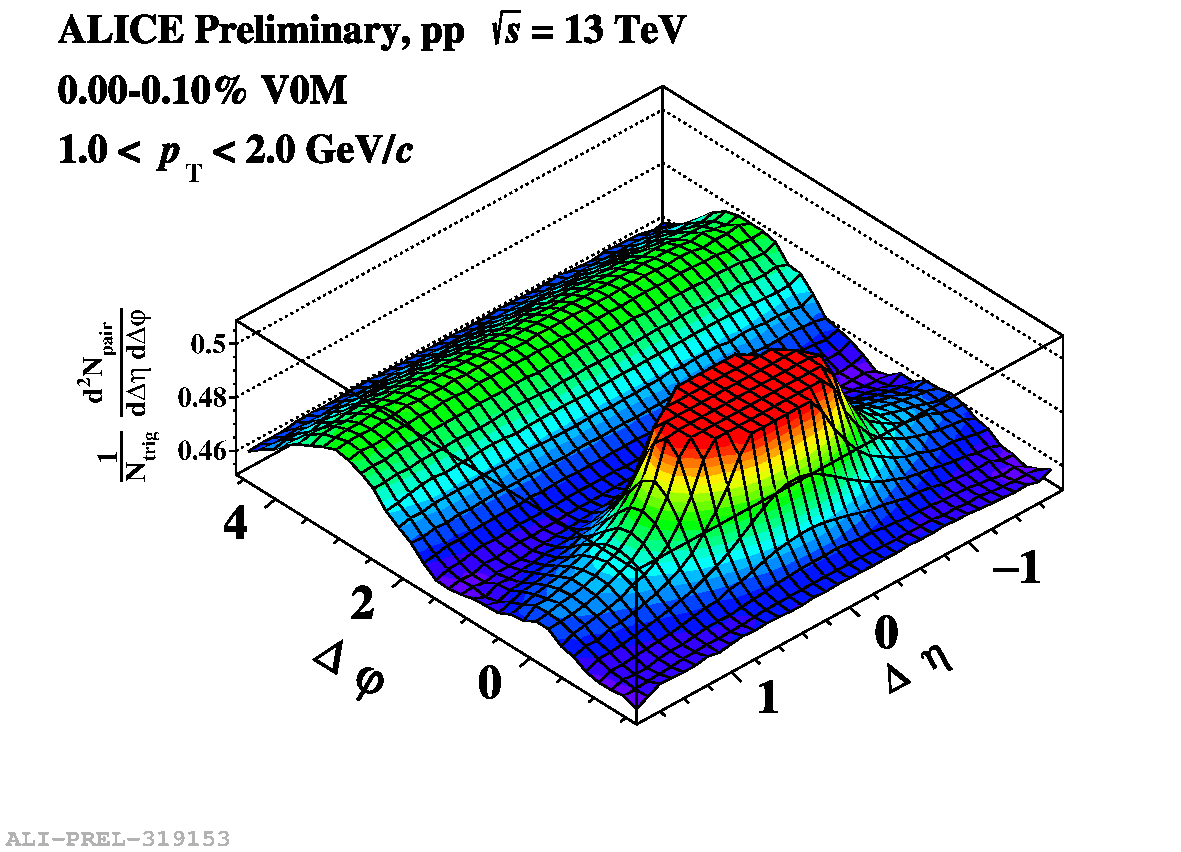
\includegraphics[width=0.47 \textwidth]{./figures/corr1.pdf} }
	\subfigure{ 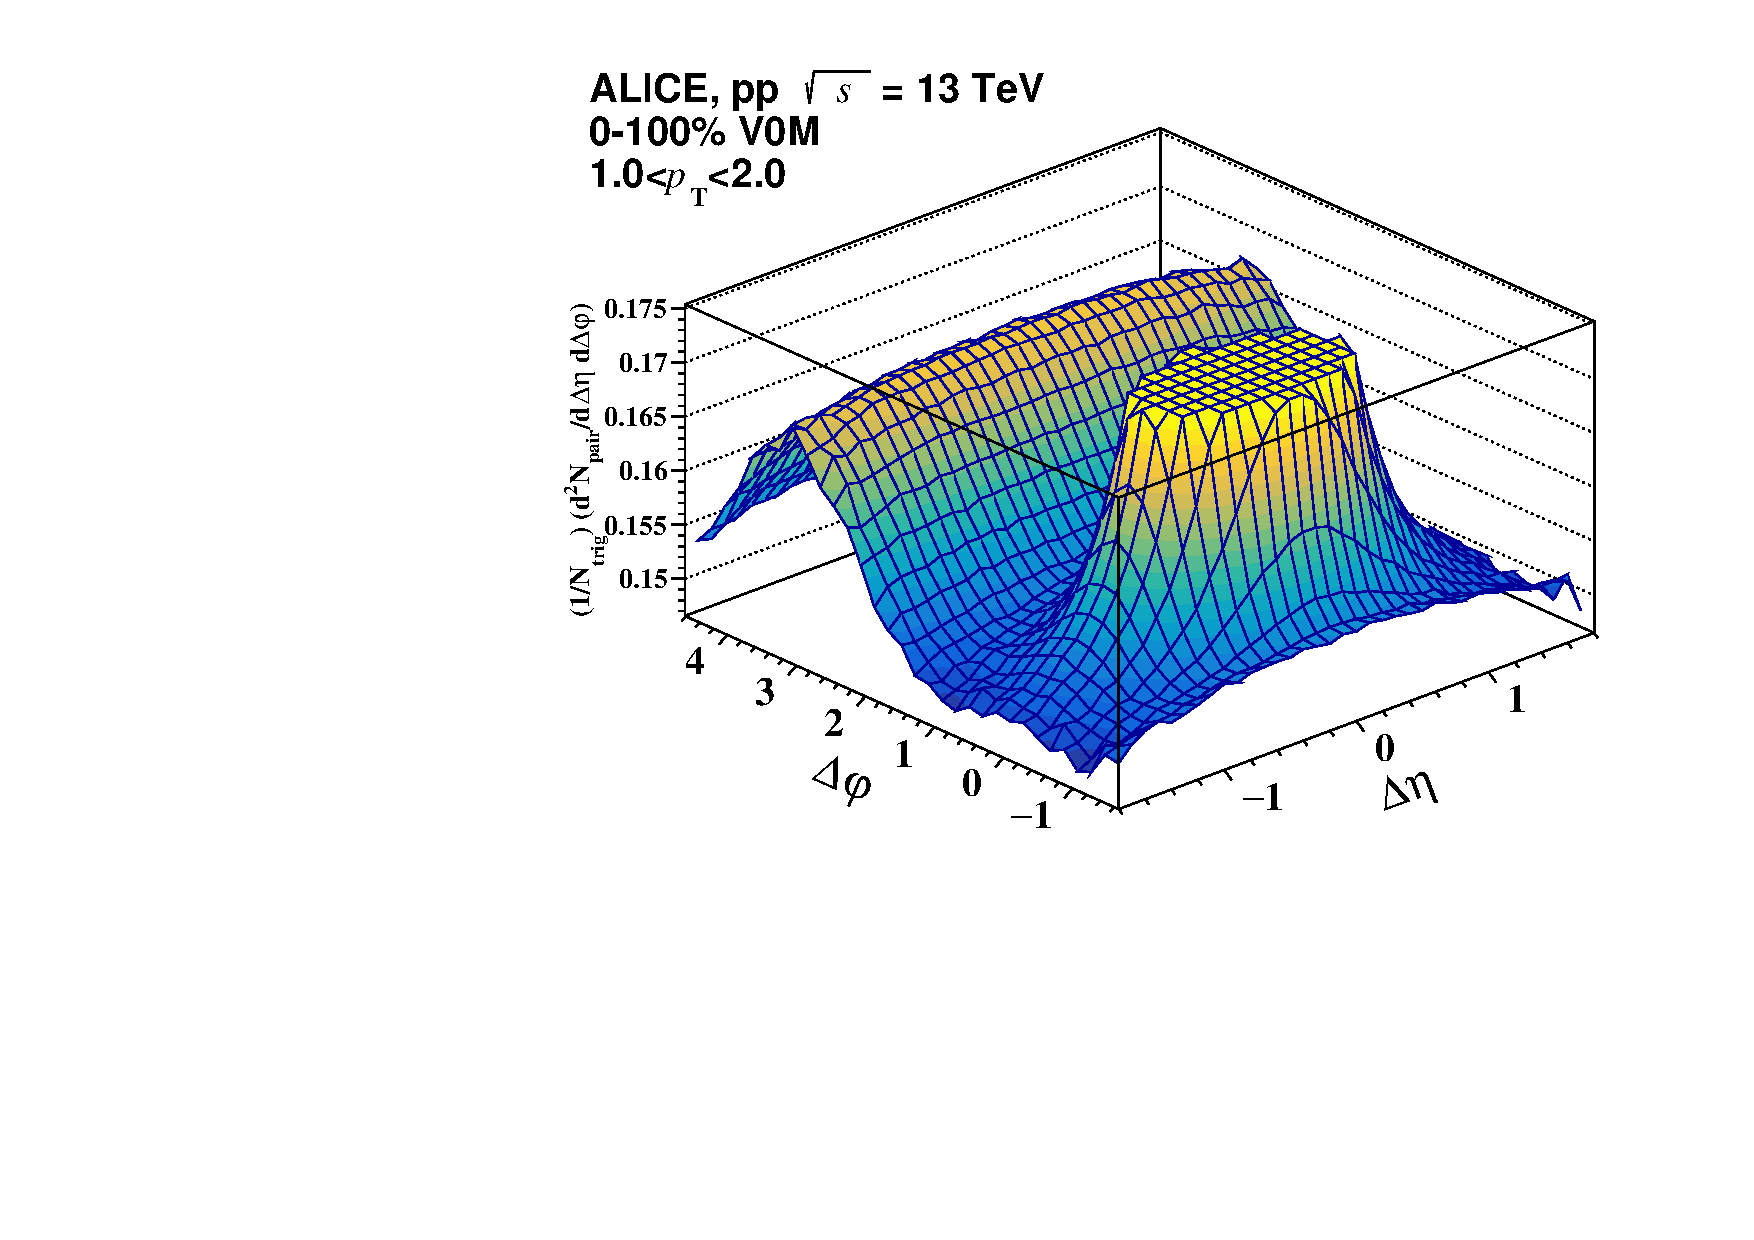
\includegraphics[width=0.47 \textwidth]{./figures/corrmb.pdf} }
	\caption{ Dihadron correlation functions as functions of $\Delta\eta$ and $\Delta\varphi$ in the high-multiplicity (0--0.1\%, left) and the minimum-bias events (0--100\%, right). The intervals of $\pttrig$ and $\ptassoc$ are equally $1 < \it{p}_{\rm{T}} < 2$ GeV/$c$. }
	\label{fig:PlotCorrMBHMT}
\end{figure}

Figure~\ref{fig:PlotCorrMBHMT} shows two-particle correlation functions as a function of the $\Delta \eta$ and $\Delta \varphi$ separation of trigger and associated particles. The per trigger yield iss measured with Eq.~\ref{eq:corrfunction} for $1 < \pttrig~\mathrm (\ptassoc) < 2$ GeV/$c$ in pp collisions at $\sqrt{\it{s}} = $\unit{13} {\rm{}TeV}. The left panel is for the high-multiplicity class. The right one is from the minimum bias events. The ridge structure is clearly observed in the high-multiplicity class while it is not seen in the minimum bias events. The away-side yield is populated mostly by correlation of jets which are back-to-back.

\begin{figure}[h!]
	\centering
	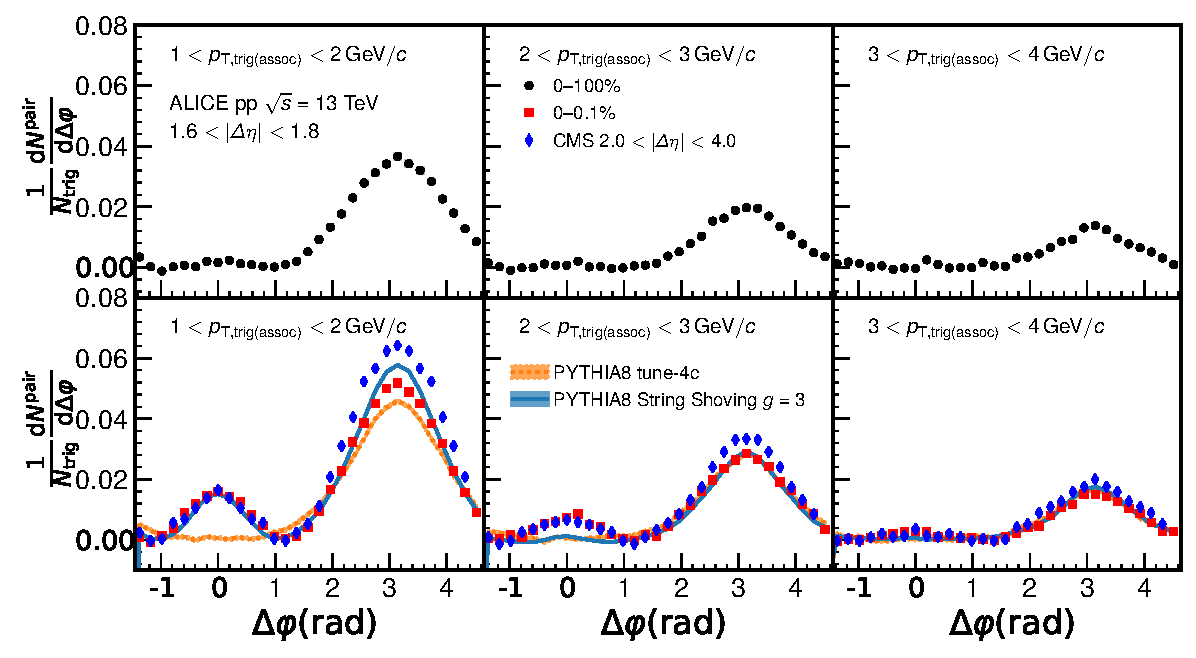
\includegraphics[width=0.9\linewidth]{./figures/Fig2_PlotDeltaPhi.pdf}
	\caption{One-dimensional $\Delta\varphi$ distribution in the large $\Delta\eta$ projection for various transverse momentum intervals in each multiplicity class. The distributions in upper panels are measured with 0--100\% multiplicity class. The distribution in lower panels are measured with 0--0.1\% multiplicity class. Transverse momentum ranges of trigger particle and associated particle are $1<\pt<2$ (left), $2<\pt<3$ (middle) and $3<\pt<4$ GeV/$c$ (right), respectively. The model predictions are presented as colored lines. Blue line corresponds to $\pythiashoving$, orange line corresponds to $\pythiam$ and green line corresponds to $\epos$.}
	\label{fig:PlotDeltaPhi}
\end{figure}
 
Projected $\Delta\varphi$ distributions of the two-particle correlation functions in $1.6<|\Delta\eta|<1.8$ are shown in Fig.~\ref{fig:PlotDeltaPhi} for various $\it{p}_{\rm{T}}$ intervals in the minimum bias class and the high-multiplicity class. The near-side ($\Delta\varphi\sim 0$) peak in high-multiplicity class is clearly observed in all transverse momentum ranges studied while there is no hint of the signal in the minimum bias class. The near-side peak is highest in the interval of $1<\it{p}_{\rm{T}}<2$ GeV/$c$ and gradually decreases with increasing $\it{p}_{\rm{T}}$ in the high-multiplicity class. The measurements in the high-multiplicity class are compared to the results measured by the CMS collaboration~\cite{Khachatryan:2015lva}. The particle multiplicity in the present analysis is estimated with the forward V0 subsystem, whereas whereas the analysis \cite{Khachatryan:2015lva}  used the mid-rapidity particles in $|\eta|<$2.4 and $\pt>0.4$ GeV/$c$. By interpolating the $\eta$ and $\pt{}$ distributions based on PYTHIA, it is found that the multiplicity in \cite{Khachatryan:2015lva} is about 20\% higher than 0--0.1\% in this analysis, corresponding 0--0.03\%. The near-side peaks in all transverse momentum ranges are comparable to each other within the uncertainties. The larger away yields observed in \cite{Khachatryan:2015lva} can be attributed to the difference in $\eta$ acceptances. The model predictions are presented for the measurements in high-multiplicity class with the identical charged track acceptance and the $\Delta\eta$ projection range to those used in this article. The high-multiplicity class for each model is determined by requiring the minimum number of charged particles larger than 105, which corresponds to the top 0--0.1\% multiplicity class based on $\pythiam$. The $\pythiashoving$ gives good estimates of the near-side peak and slightly overestimates the away-side yield for the interval of 1$<\it{p}_{\rm{T}}<$2 GeV/$c$. However the $\pythiashoving$ underestimates the near-side peak for the $\it{p}_{\rm{T}}>$2 GeV/$c$ range. $\pythiam$ does not show any peaks in the near-side as expected. It slightly underestimates the away-side peak for $1<\it{p}_{\rm{T}}<$2 GeV/$c$ and gives good estimates for the $\it{p}_{\rm{T}}>$2 GeV/$c$ range. On the other hand, $\epos$ describes better $\pt$ dependence quantitatively for the 1$<\it{p}_{\rm{T}}<$4 GeV/$c$ range, while overestimating the near-side peak for the $\it{p}_{\rm{T}}<$2 GeV/$c$ range. 


\begin{figure}[h!]
	\centering
	\subfigure{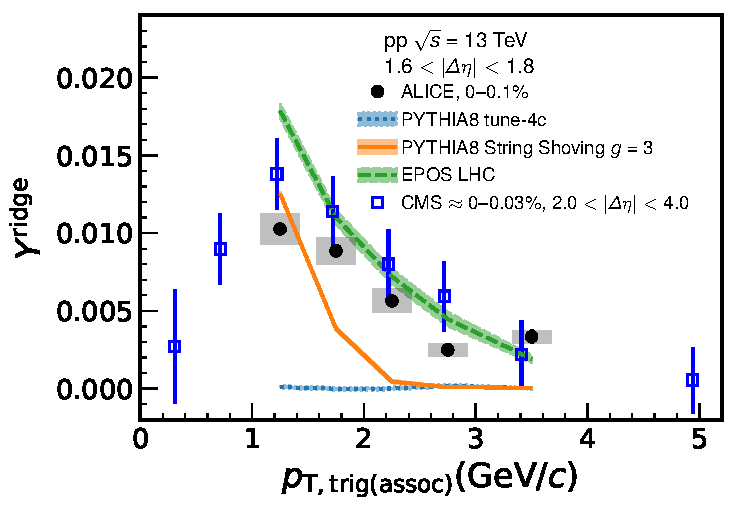
\includegraphics[width=0.99\textwidth]{./figures/Fig3_PlotRidgeYield.pdf}}
	\caption{ Fully corrected near-side ridge yield as a function transverse momentum. The filled circles denote the measurement with ALICE. The CMS measurement~\cite{Khachatryan:2015lva} is represented by open blue box markers. The three lines show model predictions from $\pythiam$ (blue line), $\pythiashoving$ (orange line) and $\epos$ (green line).}
	\label{fig:PlotYSpect}
\end{figure}

Fig.~\ref{fig:PlotYSpect} shows the near-side ridge yield measured in high-multiplicity events as a function of transverse momentum. The ALICE data are compared to \cite{Khachatryan:2015lva}.
%The ridge yields as a function of the transverse momentum are shown in Fig.~\ref{fig:PlotYSpect} in the high-multiplicity class and compared to \cite{Khachatryan:2015lva}.
Taking into account the differences in acceptance of charged tracks and estimated multiplicity, the measurements are comparable with each other. The spectrum is also compared with model calculations. $\pythiam$ gives zero yields since it does not contain the ridge effect. $\pythiashoving$ describes the yield qualitatively however its yield decreases more rapidly than the measured data as $\pttrigassoc$ increases. $\epos$, unlike $\pythiashoving$, gives estimates for the $\pt$ dependence showing the ridge yield for the $\it{p}_{\rm{T}}>2$ GeV/$c$ range, while estimating larger yield for the $\it{p}_{\rm{T}}<2$ GeV/$c$.

\subsection{Event-scale dependence of the ridge yield}
\begin{figure}[h!]
	\centering
	\subfigure{ 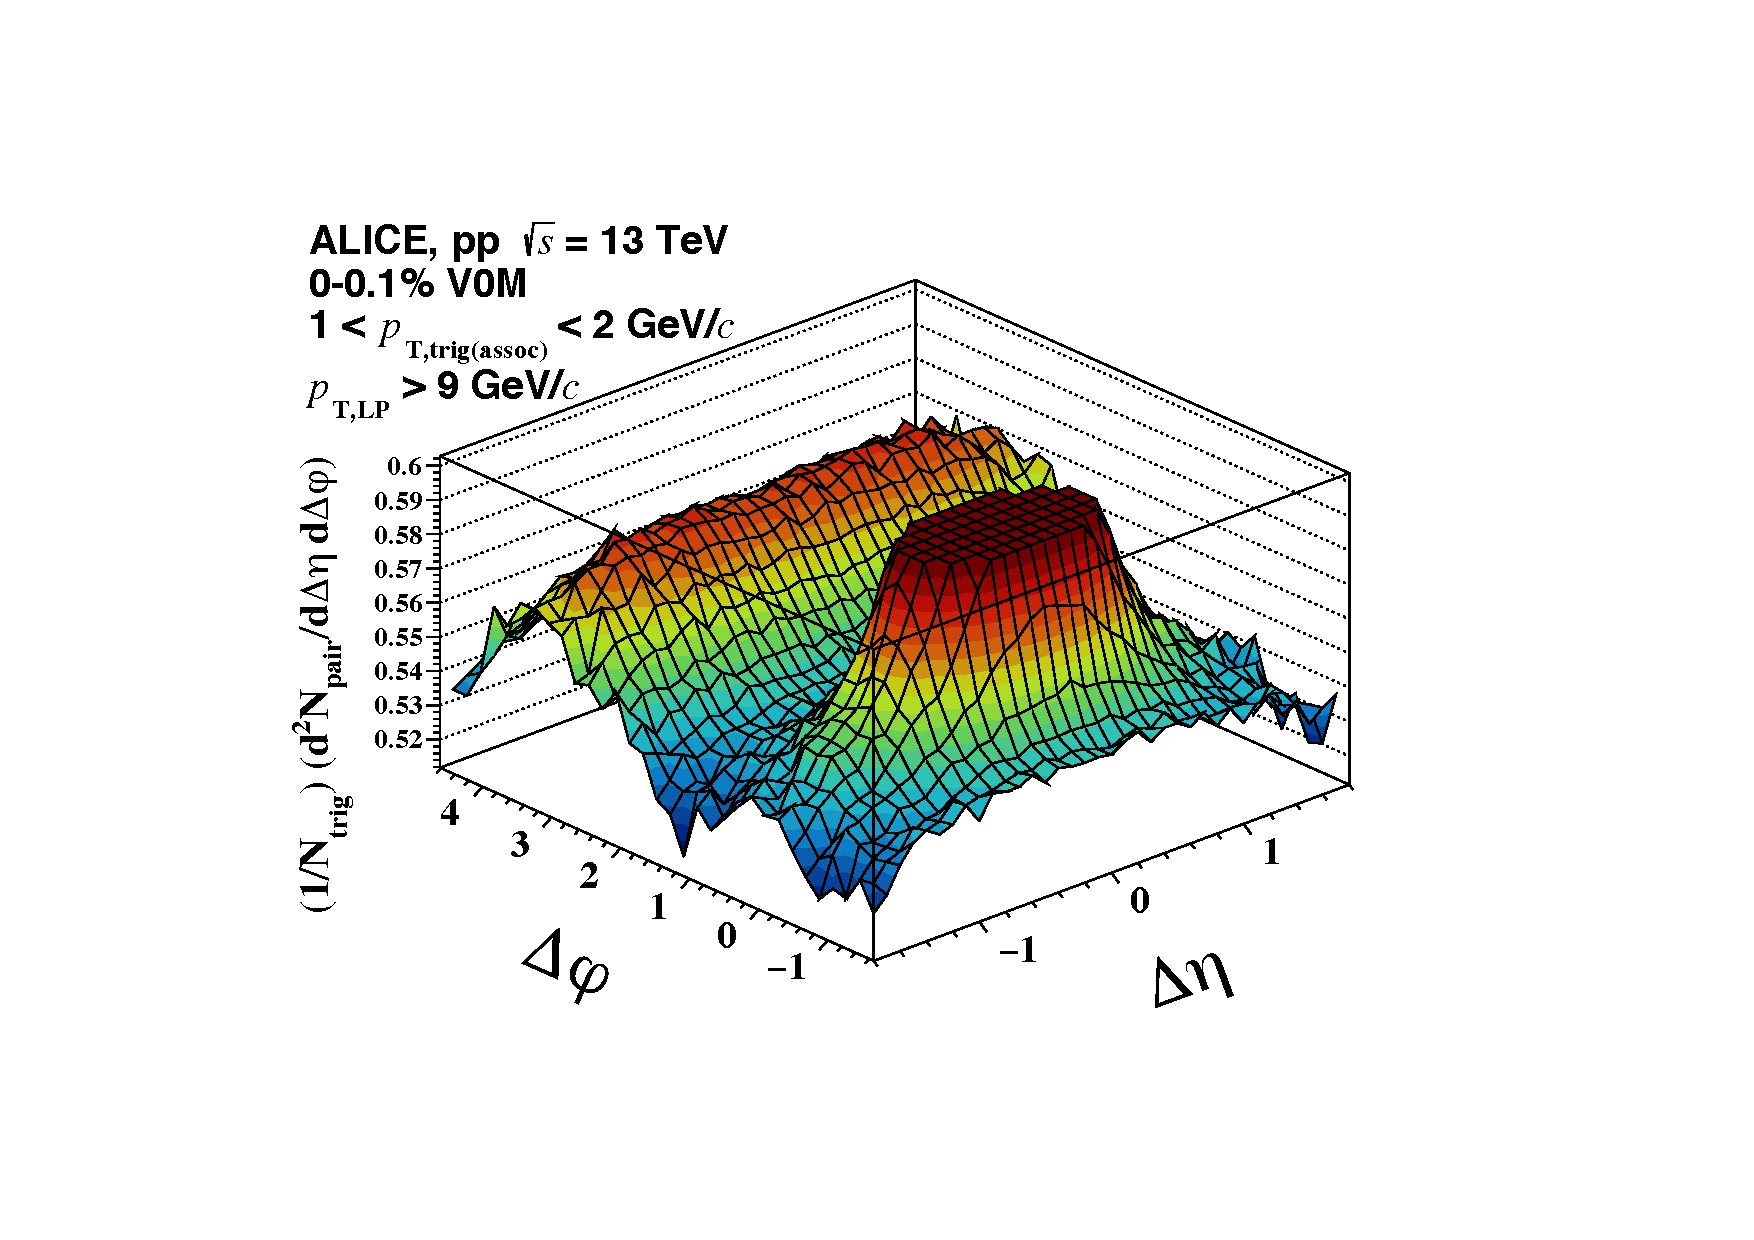
\includegraphics[width=0.47 \textwidth]{./figures/corrlh.pdf} }
	\subfigure{ 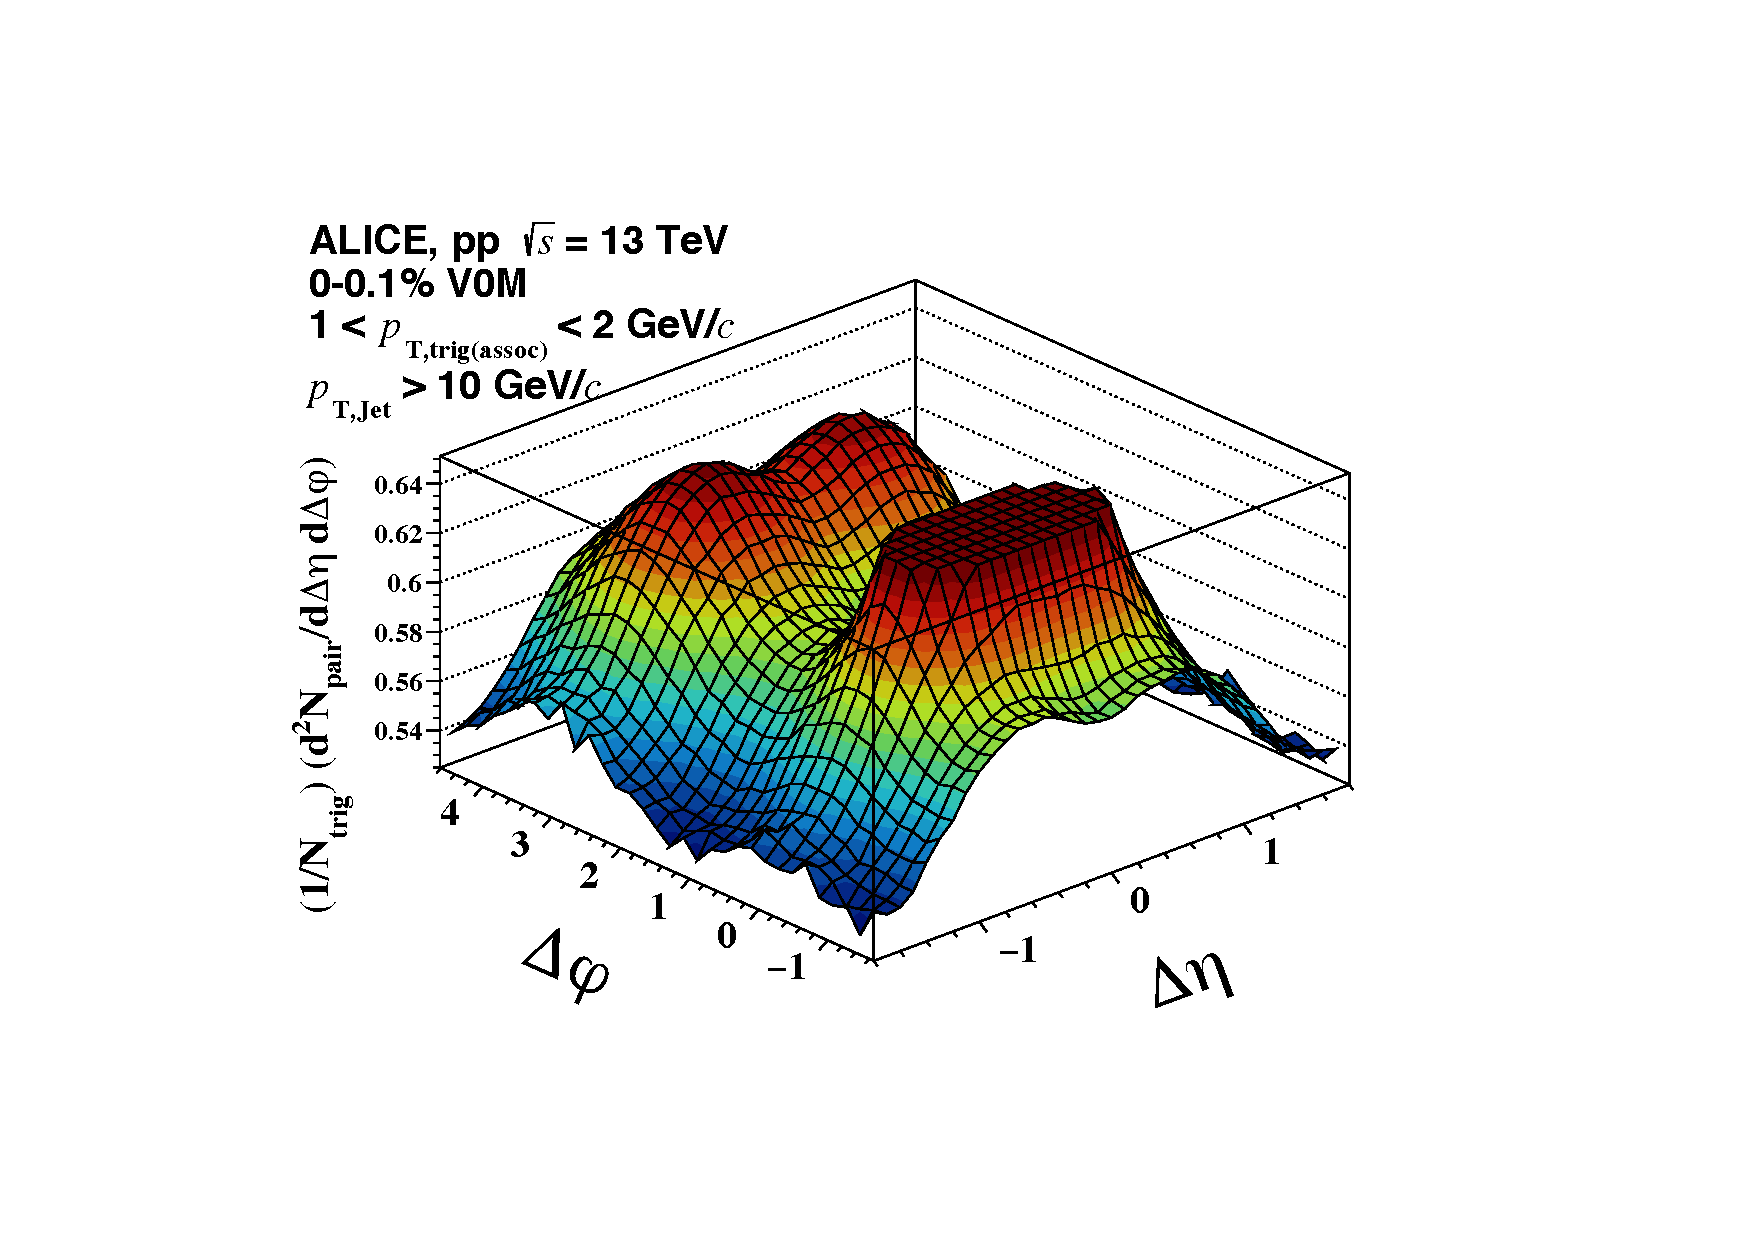
\includegraphics[width=0.47 \textwidth]{./figures/corrjet.pdf} }
	\caption{ Two-dimensional correlations function as a function of $\Delta\eta$ and $\Delta\varphi$ in top 0-0.1\% multiplicity class with the minimum $\ptlead$ (left) or $\ptjet$ (right) selection. The interval of $\pttrig$ and $\ptassoc$ is $1<\pt<2$ GeV/$c$. The minimum requirement for $\ptlead$ or $\ptjet$ is 9 or 10 GeV/$c$, respectively. }
	\label{fig:PlotCorrHMTSel}
\end{figure}

The ridge yield is further studied with respect to two different event-scales of the hard processes. Event-scale measurement by the largest $\pt$ of charged particles in each event is denoted as $\ptlead$ while the other is done by reconstructing jets and measuring their transverse momenta, represented as $\ptjet$. As shown in Fig.~\ref{fig:PlotCorrHMTSel}, the ridge structure for $1< \pttrig\,(\ptassoc) <2$ GeV/$c$ still persists in high-multiplicity pp collisions with $\ptlead>9$~GeV/$c$ (left) or $\ptjet>10$~GeV/$c$ (right) .  %The interval is the same to the measured ridge yield is maximum without the event-scale selection.
It is worth noting that the correlation function with the minimum $\ptjet$ selection has double peaks along the $\Delta\eta$ axis at $\Delta\varphi = \pi$ due to the jet tagging with the limited jet acceptance in the mid-rapidity as described in this article.

\begin{figure}[h!]
	\centering
	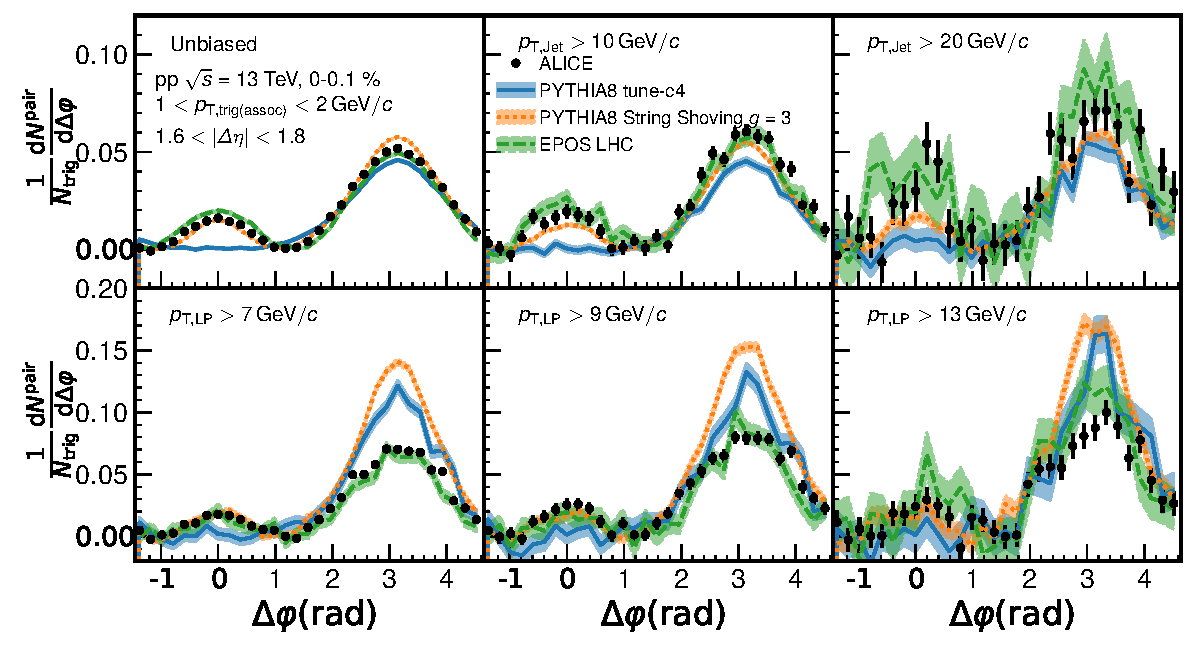
\includegraphics[width=0.99\linewidth]{./figures/Fig5_PlotDeltaPhiESE.pdf}
	\caption{ One-dimensional $\Delta\varphi$ distribution in the large $\Delta\eta$ with the minimum $\ptlead$(lower) or $\ptjet$(upper) selection for $1< \pttrig~\mathrm (\ptassoc) <2$ GeV/$c$ in the 0--0.1\% multiplicity class. The filled circles show the ALICE measurement. Model predictions are presented with a blue line for $\pythiam$, an orange line for $\pythiashoving$ and a green line for $\epos$.}
	\label{fig:PlotDeltaPhiESE}
\end{figure}

Figure~\ref{fig:PlotDeltaPhiESE} shows projected $\Delta\varphi$ distributions of the correlation functions in $1.6<|\Delta\eta|<1.8$ with the minimum $\ptlead$ (lower) and $\ptjet$ (upper) requirement. Even with the event-scale selection, the ridge is still visible at the near-side. The near-side yield increases as the threshold of $\ptjet$ increases compared to one measured in unbiased events, while the ridge yields for an increasing threshold of $\ptlead$ increase less than those of $\ptjet$. The results are compared with $\pythiashoving$, $\pythiam$, and $\epos$ calculations. The near-side peaks are qualitatively reproduced by $\pythiashoving$ and $\epos$, while underestimated by $\pythiashoving$ and overestimated by $\epos$. On the other hand, $\pythiam$ does not show the near-side peak with the event-scale selections, while giving similar estimates for away-side yield as $\pythiashoving$.
%Both models describe the away-side yield with the $\ptjet$ selection and overestimate away-side yield with the $\ptlead$ selection.

\begin{figure}[h!]
	\centering
	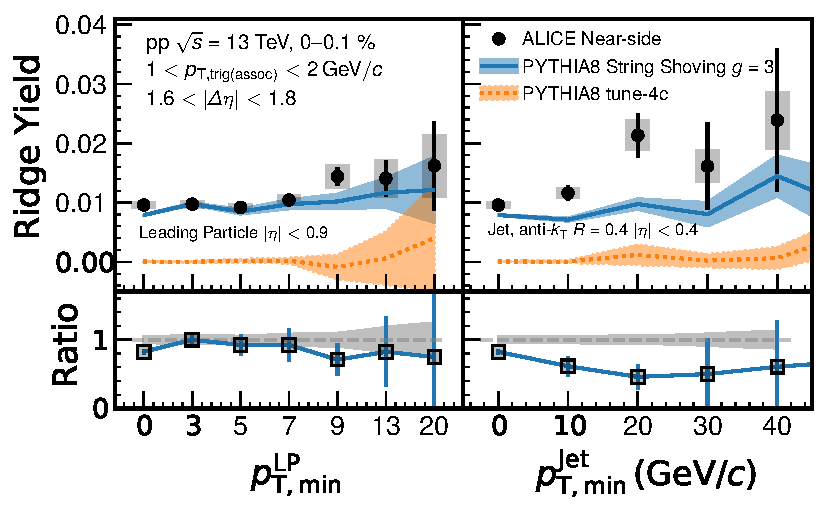
\includegraphics[width=0.99\linewidth]{./figures/Fig6_RidgeYieldESE.pdf}
	\caption{The ridge yield spectra with respect to the leading particle and jet selections. The filled circles show measurement with ALICE. Model predictions are compared to measurement as blue lines for $\pythiam$, orange lines for $\pythiashoving$ and green lines for $\epos$. Ratios of measured data to models are prepared for $\pythiashoving$ and $\epos$.}
	\label{fig:RidgeYield_ESE}
\end{figure}

Finally, the ridge yields as functions of the minimum $\ptlead$ ($\it{p}^{\rm{LP}}_{\rm{T,min}}$) and $\ptjet$ ($\it{p}^{\rm{Jet}}_{\rm{T,min}}$) selections are shown in Fig.~\ref{fig:RidgeYield_ESE}. The ridge yields are increased for $\it{p}^{\rm{LP}}_{\rm{T,min}} >$ 7 and $\it{p}^{\rm{Jet}}_{\rm{T,min}} \ge$ 10~GeV/$c$ compared to one from the unbiased events. A moderate increase of the ridge yields toward higher $\ptlead$ or $\ptjet$ is observed and there is no difference between two event selections within the uncertainties.
The results are compared with $\pythiashoving$, $\pythiam$ and $\epos$. $\pythiashoving$ describes comparable trend with data, underestimating the ridge yield. On the other hand, $\epos$ also describes comparable trend with data, overestimating the ridge yield. The origin of the enhanced ridge yields for higher momentum jet-tagged events is not clear to date but it might be related with the expected shorter impact parameters for dijet or multi-jet production events studied in~\cite{Frankfurt:2010ea}.

\begin{figure}[h!]
	\centering
	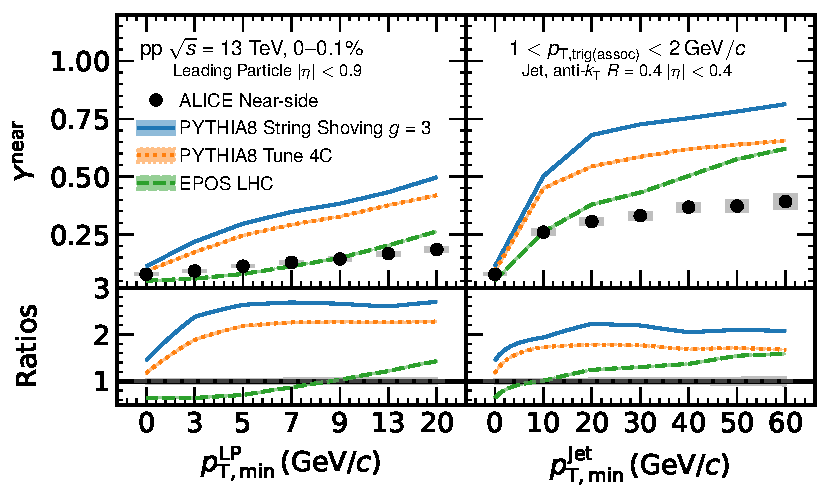
\includegraphics[width=0.99\linewidth]{./figures/Fig9_JetYieldESE.pdf}
	\caption{The jet yield spectra with respect to the leading particle (left) and jet selections (right). The filled circles show measurement with ALICE. Model predictions are compared to measurement as blue lines for $\pythiam$, orange lines for $\pythiashoving$ and green lines for $\epos$.}
	\label{fig:RidgeYield_ESE}
\end{figure}

Jet yield has been measured as a function of minimum $\ptlead$ and $\ptjet$ threshold to further discuss ridge yields and jet yields.
%quantify the trend of the jet yield.
$\epos$ provides comparable estimates for jet yields, while $\pythiam$ and $\pythiashoving$ overestimate jet yields for both selections. Increasing trend of jet yield as a function of minimum $\ptlead$ and saturating trend of jet yield as a function of minimum $\ptjet$ have been observed and estimated by models. Jet yield measured with $\ptlead>$20~GeV/$c$ is comparable with the one measured with $\ptjet>$10~GeV/$c$, where ridge yields with corresponding selections are also comparable.